\documentclass{article}

\usepackage[utf8]{inputenc}
\usepackage[T1]{fontenc}
\usepackage[a4paper, margin=1in]{geometry}
\usepackage{amsmath}
\usepackage{graphicx}
\usepackage{listings}
\usepackage{xcolor}
\usepackage{tcolorbox}
\usepackage{scalerel}
\usepackage{bav4}


\title{Livrable 5}
\author{
Amberny Peran, Barnouin Clement, Burellier Loucas, \\
Krainik-Saul Vladimir, Schicke Samuel, 
}
\date{\today}

\begin{document}

\maketitle

\tableofcontents
\clearpage


\section{Introduction}
MiniCoffee est un groupe français spécialiste de l’univers du café, connu notamment pour ses machines à café en libre service. Pour l’année 2025, l’entreprise souhaite mettre à jour son infrastructure réseau interne en ajoutant : 
\begin{itemize}
    \item Divers serveurs d’utilité interne pour les employés et l'équipe informatique;
    \item Un réseau invité pour permettre à ses fournisseurs d’utiliser du matériel informatique sur place;
    \item Divers serveurs accessibles en ligne (site Web, serveur DNS public);
    \item Une meilleure communication entre ses machines à café et son infrastructure, qui a été un des points faibles de l’entreprise ces dernières années.
\end{itemize}
Pour cette tâche, MiniCoffee a fait appel à BAV4, notre équipe d’étudiants de l’IUT2 Informatique de Grenoble.

\section{Architecture}
L'architecture de notre réseau n'a pas énormément changé. 
Les seules modifications apportées au réseau sont : 
\begin{itemize}
    \item Passage d'un LAN à un VLAN pour une meilleure segmentation du réseau.
    \item Les adresses IP internes se terminent par 1XX.
    \item Les adresses IP externes se terminent par XX.
\end{itemize}

\begin{figure}
    \centering
    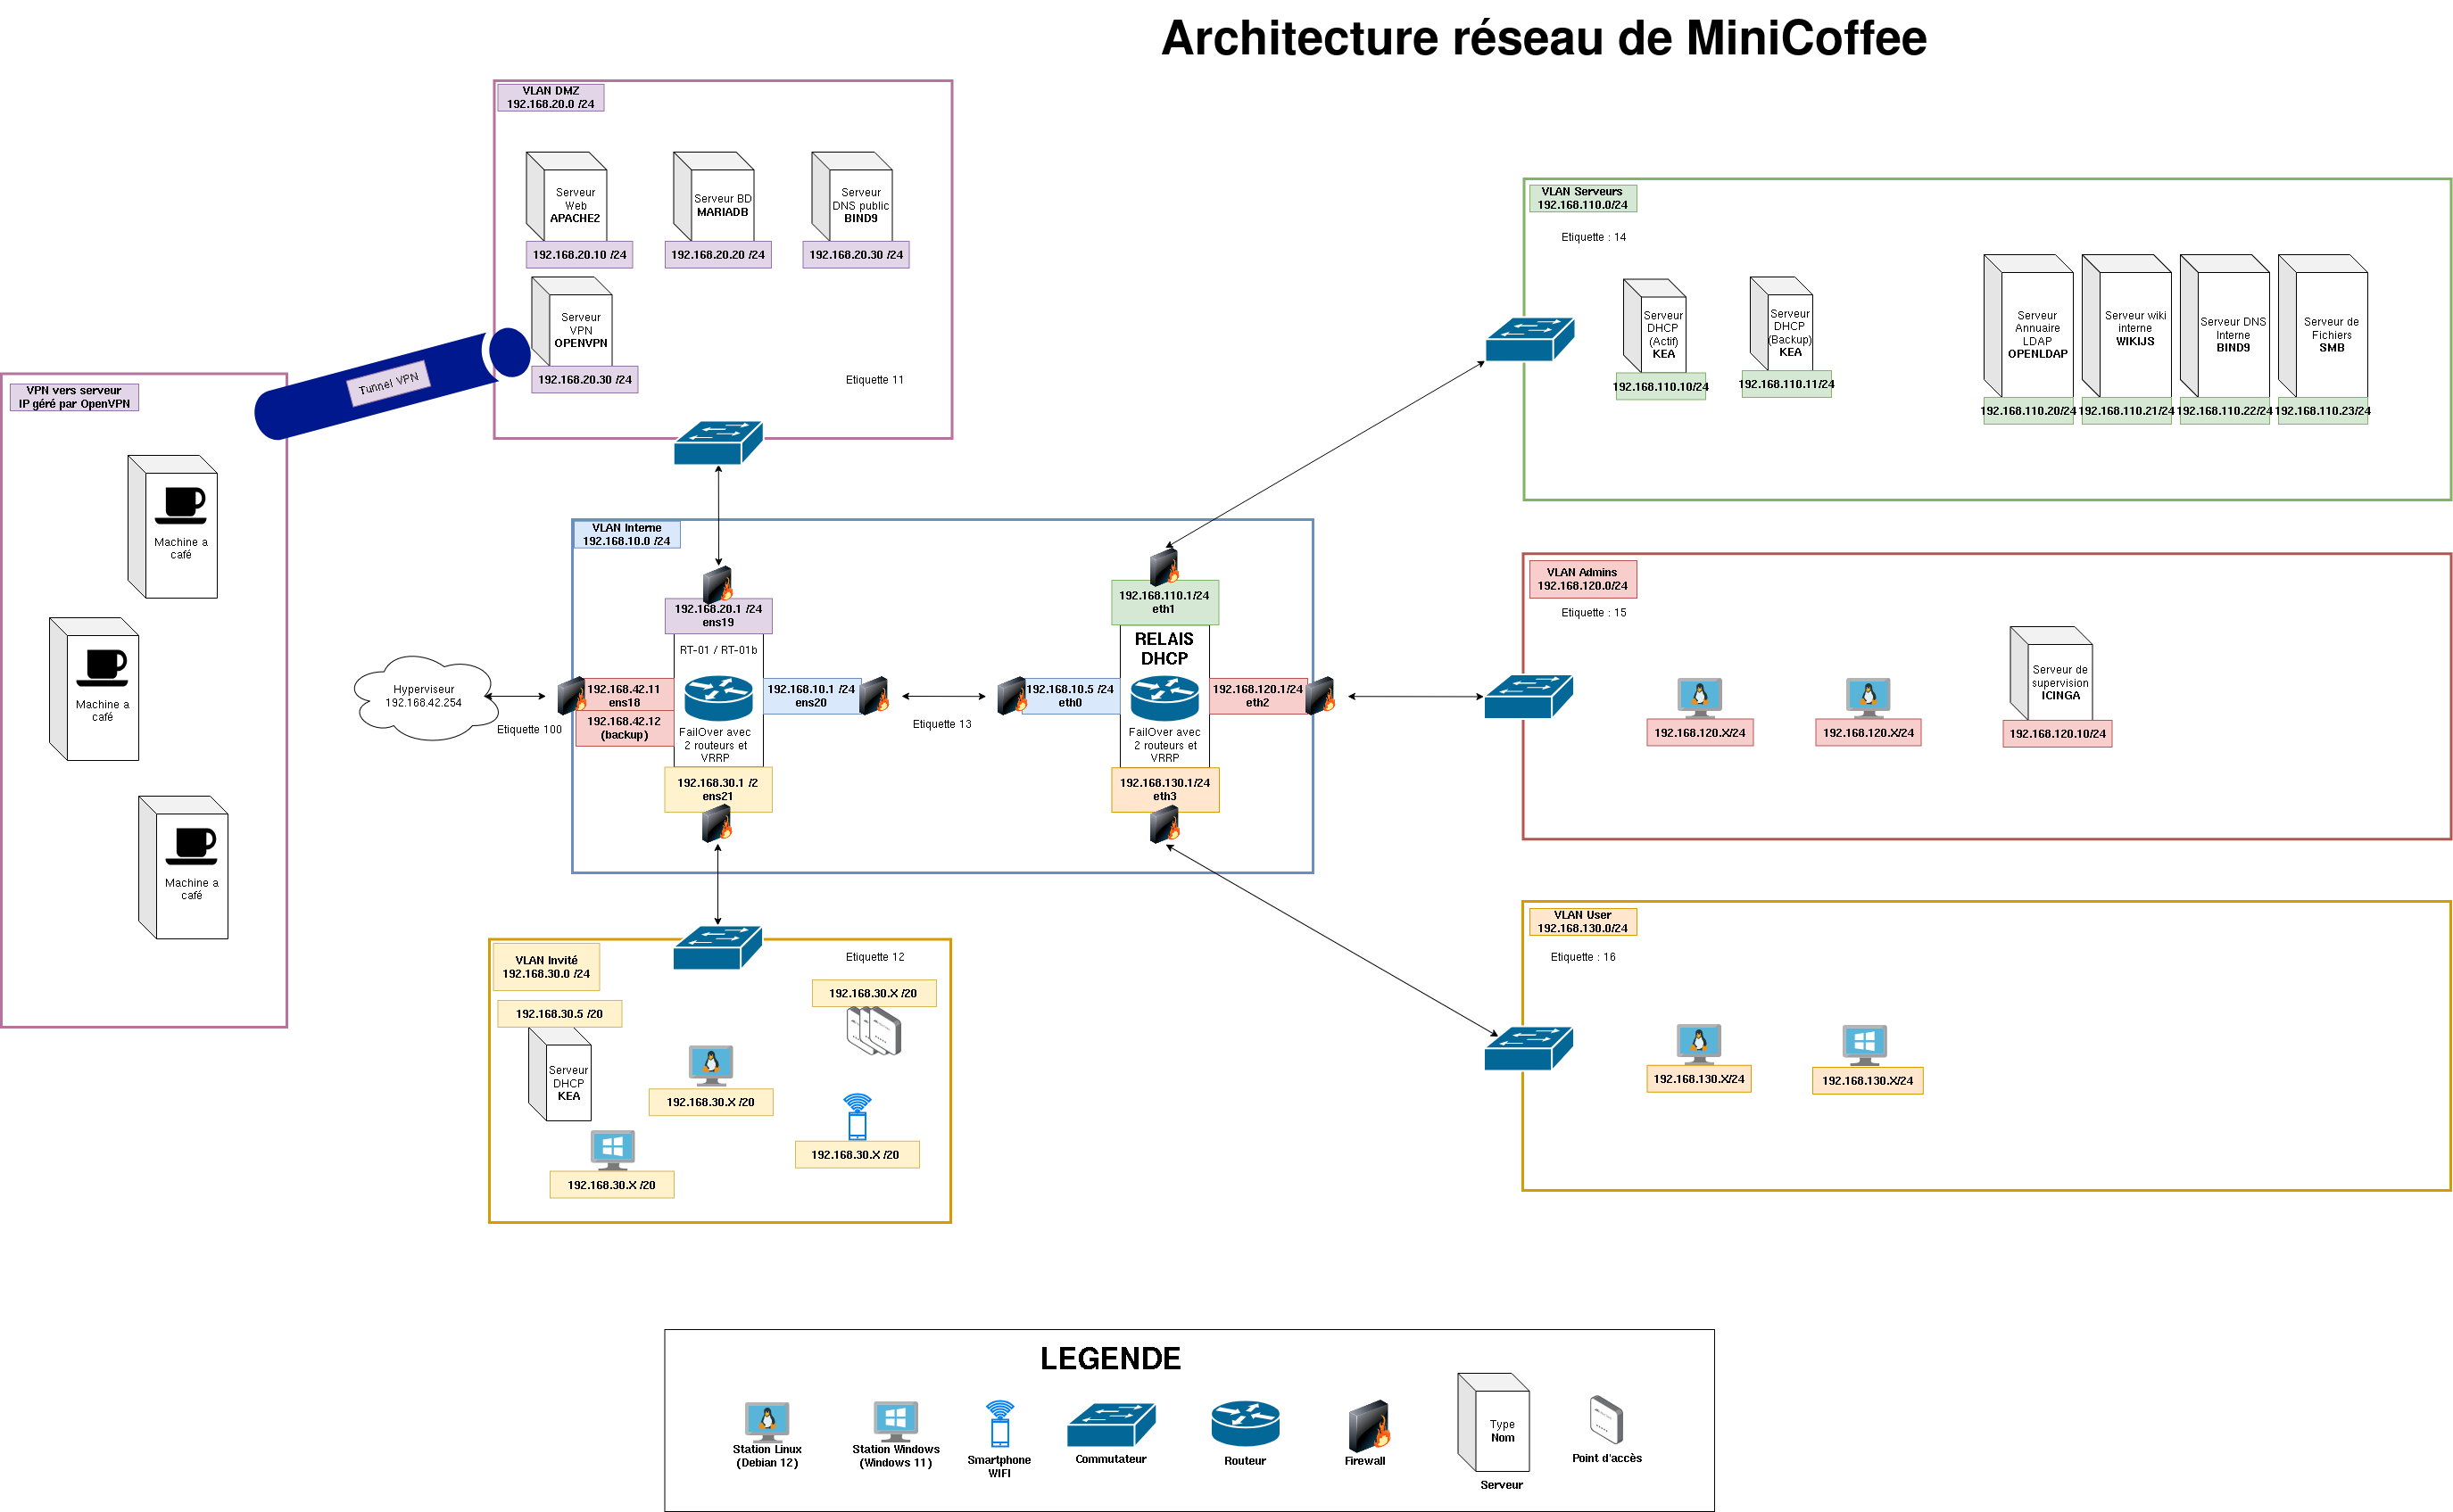
\includegraphics[angle=-90, width=1\textwidth, trim=0 0 0 2.3cm, clip]{../assets/Architecture.drawio.png}
    \caption{Architecture réseau de MiniCoffee}
\end{figure}

\clearpage

\section{Ressources Matérielles utilisées}
Actuellement, notre infrastructure réseau comprend un total de 9 machines actives, chacune jouant un rôle spécifique dans notre environnement.
\\

En ce qui concerne le stockage, nous allouons entre 3 et 5 Go d’espace disque par machine, en fonction de leurs besoins en ressources et des tâches qu’elles doivent accomplir. Plus précisément :
\begin{itemize}
    \item Les machines nécessitant le moins de ressources se voient attribuer 3 Go de stockage, ce qui est suffisant pour assurer leur bon fonctionnement sans surconsommation d’espace.
    \item Les machines les plus sollicitées, qui traitent des volumes de données plus importants ou exécutent des processus plus intensifs, bénéficient quant à elles de 5 Go de stockage afin de garantir des performances optimales.
\end{itemize}

En termes de mémoire vive (RAM), chaque machine de notre réseau dispose actuellement de 1 Go. Cette allocation permet de répondre aux besoins de nos applications tout en maintenant un bon équilibre entre performance et consommation de ressources.
\\

Nous surveillons régulièrement l’utilisation de la RAM et du stockage afin d’optimiser notre infrastructure si nécessaire et d’anticiper toute montée en charge.

\section{Installation et Configuration des éléments de l'infrastrucure}
Nous allons détailler dans cette partie comment nous avons configuré les éléments de notre infrastructure réseau.
\subsection{Résaux Virtuel}

Nous avons créé des VXLAN pour interconnecter les hyperviseurs au sein du cluster, permettant ainsi une communication entre eux. De plus, nous avons mis en place des VNET spécifiques pour chaque hyperviseur afin de segmenter et d’optimiser la gestion du réseau virtuel, garantissant une meilleure performance et une isolation accrue des ressources.

\subsection{Routeurs}
\subsubsection{Configuration des interfaces}
Tout d'abord, il faut configurer les interfaces de la machine qui va servir de routeur.

Il faut configurer le fichier \textbf{/etc/network/interfaces} pour attribuer les bonnes ip et CIDR pour chaque interface. Voici un explique de chaque paramètre que l’on peut mettre :

\newpage



Voici un fichier de configuration type pour un routeur avec plusieurs interfaces :

\begin{configbox}{/etc/network/interfaces}
    \begin{lstlisting}
        # Interface WAN (connectee a Internet)
        auto eth0
        iface eth0 inet dhcp
        mtu 1450  # Taille MTU standard
        # Interface LAN 1 
        (reseau interne 192.168.1.0/24)
        auto eth1
        iface eth1 inet static
            address 192.168.1.1/24
            gateway 192.168.1.254  
            # Facultatif, utilise uniquement si ce reseau doit 
            sortir par une autre route
            dns-nameservers 192.168.1.1 8.8.8.8
            dns-domain lan1.local
            mtu 1450  # Optimise pour les reseaux 
            locaux rapides

        # Interface LAN 2 
        (reseau interne 10.10.0.0/24)
        auto eth2
        iface eth2 inet static
            address 10.10.0.1/24
            mtu 1450  # Optimise pour un second 
            reseau local

        # Activation du routage entre les reseaux
    post-up echo 1 > /proc/sys/net/ipv4/ip_forward

        # Ajout de routes pour permettre aux 
        deux reseaux de communiquer entre eux
        # Ajout de routes pour permettre aux 
        deux reseaux de communiquer entre eux
    post-up ip route add 192.168.1.0/24 
    via 192.168.1.1 dev eth1 
    post-up ip route add 10.10.0.0/24 
    via 10.10.0.1 dev eth2 
    \end{lstlisting}
\end{configbox}
\paragraph{Détail de la configuration}
\begin{itemize}
    \item Une première ligne avec la façon d’on l’interface s’active.
    \begin{itemize}
        \item (L2) \monosp{auto [nomInterface]}  : Pour activer automatiquement au démarrage. Idéal pour les interfaces fixes, comme celles des serveurs.
        \item \monosp{allow-hotplug [nomInterface]} : Pour activer uniquement quand elle est détectée. Idéal pour les interfaces amovibles.
    \end{itemize}
    \item Une seconde qui définit sa configuration.
    \begin{itemize}
        \item \monosp{iface eth0 inet manual} : Interface n'a pas de configuration IP et doit être activé à la main
        \item \monosp{iface eth0 inet none} : Interface active mais sans configuration IP
        \item (L3) \monosp{iface [nomInterface] inet dhcp} : Utilise le DHCP pour l'attribution d'IP, ...
        \item (L8) \monosp{iface eth1 inet static} : Pour faire une configuration avec une IP statique
    \end{itemize}
    \item Ajout de paramètres pour la configuration de IP si configuration \monosp{static} :
    \begin{itemize}
        \item (L9) \monosp{address 192.168.1.1/24} : L'adresse IP static
        \item (L10) \monosp{gateway 192.168.1.254} : Le gateway
        \item (L13) \monosp{dns-nameservers 192.168.1.1 8.8.8.8} : Les DNS
        \item (L14) \monosp{dns-domain lan1.local} : Le domaine DNS
        \item \monosp{metric 10} : La priorité de l'utilisation de cette interface. Plus la valeur est basse, plus la priorité est haute.
        \item \monosp{up ip addr add 192.168.100.15/24 dev [nomInterface]} : Si l'on souhaite plusieurs adresses IP sur la même interface
        \item (L4) \monosp{mtu 1450} : MTU maximum
        \item (L33) \monosp{post-up ip route add 192.168.1.0/24 via 192.168.100.10} : Si la machine doit accéder à un réseau via une passerelle spécifique. Tout le trafic vers 192.168.200.0/24 passera via 192.168.100.10.
    \end{itemize}
\end{itemize}

Une fois le fichier configuré, il redémarrer le service avec 
\rootcmd{systemctl restart networking.service}

\subsubsection{Configuration des routes entre les réseaux}
\com{Pas sur de l'explication les sangs ?}
Par défaut, une machine Linux ne fait pas passer n'importe quel paquet \com{c'est le but d'avoir des routeurs ?} comme doit le faire un routeur. On doit donc activer cette fonctionnalité qui est sous la forme d'un option dans le fichier \textbf{/etc/sysctl.conf}.

\begin{command}
    sysctl -p /etc/sysctl.conf
\end{command}

\com{<La partie qui suit devrait être dans les routeurs non ?}
Mettre en place le NAT (fichier nft a executer) 
\begin{codebox}{filtrage-nat}
\begin{lstlisting}[language=Bash]
nft add table filtrage_nat
nft 'add chain filtrage_nat prerouting { type nat hook prerouting priority 0 ; }'
nft 'add chain filtrage_nat postrouting { type nat hook postrouting priority 0 ; }'
nft add rule filtrage_nat postrouting masquerade
\end{lstlisting}
\end{codebox}

\subsection{Serveur DHCP}
Afin de pouvoir attribuer des @IP de façon automatique, nous allons installer un serveur DHCP, le logiciel que nous allons utiliser pour le DHCP s'appelle \monosp{Kea}. Kea est un serveur DHCP développé par l'ISC, conçu pour être plus flexible et performant que ISC DHCP. Kea supporte IPv4 et IPv6 et est particulièrement adapté aux environnements à grande échelle nécessitant une gestion avancée des adresses IP


\subsubsection{Installation}
\begin{itemize}
    \item Nous créons une VM avec une @IP statique car c’est cette dernière qui attribuera les @IP.
    \item Installation de Kea : \rootcmd{apt install kea-dhcp4-server}
\end{itemize}

\subsubsection{Configuration}
\begin{itemize}
    \item Nous sauvegardons la configuration pour la restaurer en cas de problème 
    \rootcmd{mv /etc/kea/kea-dhcp4.conf /etc/kea/kea-dhcp4.conf.bkp}
    \item Nous créons par la suite le fichier \monosp{/etc/kea/kea-dhcp4.conf} qui doit contenir la configuration suivante :
\end{itemize}
    \newpage
\begin{configbox}{/etc/kea/kea-dhcp4.conf.bkp}
    \begin{lstlisting}
{
"Dhcp4": {
	"interfaces-config": {
		"interfaces": [
			"ens18"
		]
	},
	"valid-lifetime": 691200,
	"renew-timer": 345600,
	"rebind-timer": 604800,
	"authoritative": true,
	"lease-database": {
		"type": "memfile",
		"persist": true,
		"name": "/var/lib/kea/kea-leases4.csv",
		"lfc-interval": 3600
	},
	"subnet4": [
		{
			"subnet": "192.168.120.0/24",
			"pools": [
				{
					"pool": "192.168.120.10 - 192.168.120.200"
				}
			],
			"option-data": [
				{
					"name": "domain-name-servers",
					"data": "192.168.110.22"
				},
				{
					"name": "domain-search",
					"data": "bav4.local"
				},
				{
					"name": "routers",
					"data": "192.168.120.1"
				}
			]
		},
[... Ajouter autant de subnet que de sous reseaux sont concernes]
	]
}
}
    \end{lstlisting}
\end{configbox}
\paragraph{Détail de la configuration}
\begin{itemize}
	\item (L2) \monosp{"Dhcp4"} : Indique que l'attribution est faite avec des @IPv4
	\item (L3-5) Indique l'interface qui emettra les DHCP response
	\item (L8-11) Configuration des differents temps de sauvegarde/renouvellement...
	\item (L12-17) Configuration de la base de donnée qui contiendras les données DHCP
	\item (L18) \monosp{"subnet4"} : Indique que le subnet spécifié est en IPv4
	\item (L20) \monosp{ "subnet": "192.168.14.0/24"} : indique le sous reseau ou le serveur DHCP attribue les adresses.
	\item (L21-26) Configure les differents intervalles IP attribués
	\item (L27-L39) Configure les options DHCP (@IP du serveur DNS, adresse du serveur DNS, @IP du routeur)
\end{itemize}

\subsection{Serveur DNS}
Afin de pouvoir lier un nom a une machine, nous allons installer des serveurs DNS (Domain Name Server), ces derniers feront le lien entre les @IP des différentes machines et le nom que nous leur avons attribué. Le logiciel en charge du DNS s'appelle \monosp{BIND 9}. BIND 9 est un serveur DNS open source développé par l’ISC. Il est reconnu pour sa stabilité, sa sécurité et sa compatibilité avec les standards du DNS. Doté de nombreuses fonctionnalités avancées, il prend en charge DoT (DNS over TLS), le contrôle d’accès, la journalisation fine, ainsi que la gestion en mode maître/esclave. BIND 9 est configurable via des fichiers texte et s’adapte aussi bien aux petits réseaux qu’aux infrastructures de grande taille

\paragraph{Marche a suivre :}
\begin{enumerate}
	\item Nous allons créer 2 serveur DNS, un serveur Externe, qui va être accessible depuis l’exterieur, et un serveur DNS Interne, qui va être accessible uniquement depuis l’interieur, ca sera utile pour le wiki. 
	\item Nous allons commencer par créer le DNS privé puis nous le cloneront pour en faire un DNS public, il faudra juste supprimer les alias créés pour le wiki, supprimer l’ACL “lan” et l’option lan dans allow-query (voir suite)
\end{enumerate}

\subsubsection{Installation de BIND9}
Nous installons Bind9 via apt avec la commande suivante :
\rootcmd{apt install bind9 dnsutils}

\subsubsection{Configuration des options DNS}
Nous allons d'abord copier la configuration pour pouvoir la rétablir facilement en cas d'erreur :
\rootcmd{cd /etc/bind }
\rootcmd{cp named.conf.options named.conf.options.bkp}
\rootcmd{cp named.conf.local named.conf.local.bkp} 

Nous allons ensuite modifier le fichier de config \monosp{/etc/bind/named.conf.options} qui contient les options du serveur DNS.	
\begin{configbox}{/etc/bind/named.conf.options}
\begin{lstlisting}
acl "lan" {
	192.168.110.0/24;
	192.168.120.0/24;
	192.168.130.0/24;
	localhost;
	localnets;
};
options{ 
	forwarders{
		152.77.1.22
	}
	allow-query { lan; }; 
};
\end{lstlisting}
\end{configbox}
\paragraph{Détail de la configuration}
\begin{itemize}
	\item (L1) \monosp{acl "lan"} : On déclare une ACL appellée "lan", qui permet que seule les @Ip spécifiées auront accès au serveur DNS
	\item (L2-7) Déclarations des sous-réseaux concernés par l'ACL
	\item (L9-11) On change le forwarder (le serveur DNS qui résoudra les noms si le nôtre ne les contient pas) par le DNS de l'UGA
	\item (L12) \monosp{allow-query { lan; };} indique que seuls les sous-réseaux de l'ACL peuvent query le serveur DNS
\end{itemize}

\subsubsection{Configuration de zone} 
Nous allons desormais créer la zone bav4.local, c'est cette derniere qui contiendra les enregistrements dns (par exemple wiki.bav4.local). Dans \monosp{/etc/bind/named.conf.local}, nous ajoutons donc la zone suivante:

\begin{configbox}{/etc/bind/named.conf.local}
\begin{lstlisting}
zone "bav4.local" {
    type master;
    file "/etc/bind/db.bav4.local";
    allow-update { none; };
};
\end{lstlisting}
\end{configbox}
\paragraph{Détail de la configuration}
\begin{itemize}
	\item (L2) Indique que ce serveur DNS est l'autorité principale (ou maître) pour la zone bav4.local.
	\item (L3) Indique l'emplacement du fichier qui contient les enregistrements (voir suite)
	\item (L4) Interdit toute mise à jour dynamique des enregistrements DNS pour la zone concernée.
\end{itemize}

Nous allons ensuite dupliquer le fichier \monosp{db.local} en l’appellant db.bav4.local pour pouvoir configurer la zone : 
\rootcmd{cp /etc/bind/db.local /etc/bind/db.bav4.local}
Puis, dans \monosp{db.bav4.local}, nous allons mettre en place la config suivante :
\label{subsubsec:confzonedns}
\begin{configbox}{/etc/bind/named.conf.local}
\begin{lstlisting}
$TTL    604800
@       IN     SOA    srv-dns.bav4.local.  root.bav4.local. (
                              1         ; Serial
                         604800         ; Refresh
                          86400         ; Retry
                        2419200         ; Expire
                         604800 )       ; Negative Cache TTL
;
@               IN      NS      srv-dns.bav4.local.
srv-dns         IN      A       192.168.110.22
ldap			IN		A		192.168.110.30

[... ajouter autant d'enregistrement que necessaire]
\end{lstlisting}
\end{configbox}
\paragraph{Détail de la configuration}
\begin{itemize}
	\item (L3) Numéro de serie
	\item (L4) Délai de rafraichissement pour la synchronisation des configurations entre plusieurs serveurs DNS
	\item (L5) Délai au bout duquel un serveur DNS secondaire devra retenter une synchronisation
	\item (L6) Temps d'expiration du serveur DNS
	\item (L7) Durée de conservation dans le cache de l'information "NXDOMAIN"
	\item (L9-LXX) Création des enregistrement DNS : plusieurs formes possibles :
	\begin{enumerate}
		\item \textbf{Lien nom-@IP :}	<nom-de-l'hote>   	IN	A		<@IP>
		\item \textbf{Lien alias-nom :}	<nom-de-l'alias> 	IN	CNAME 	<nom-de-l'enregistrement-de-référence>
	\end{enumerate}		  
\end{itemize}

Une fois cela fait, relançons \monosp{bind9} et notre serveur DNS est maintenant opérationnel :
\rootcmd{systemctl restart bind9}
\rootcmd{systemctl enable named.service}

Pour le vérifier, utilisons la commande suivante :
\cmd{nslookup google.com}

\subsubsection{Configuration de DoT (DNS over TLS}
Afin de rajouter une couche de sécurité dans les requetes DNS, nous allons utiliser DoT (DNS over TLS) qui permet de chiffrer nos requetes DNS. Nous utiliseront par la suite \monosp{systemd-resolved} du coté client.

\paragraph{Niveau Serveur\\}
\monosp{bind9 v9.18.33} supporte DoT sans besoin d'un logiciel tiers de type proxy, nous allons donc le mettre en place directement dans bind9.
\begin{enumerate}
	\item Nous créons et se place dans un nouveau dossier \monosp{ssl}
\rootcmd{cd /etc/bind/ssl}
	\item Nous générons une clé et un certificat (auto-signé), nécessaires pour TLS :
\rootcmd{openssl req -x509 -newkey rsa:2048 -nodes -keyout /etc/bind/ssl/cleDNS.key -out /etc/bind/ssl/certDNS.crt -days 365 -subj "/CN=bav4.local"
}
	\item Nous donnons ensuite l'ownership de la clé a \monosp{bind}
\rootcmd{chown bind:bind /etc/bind/ssl/cleDNS.key}
	\item Finalement, nous modifions le fichier de configuration \monosp{/etc/bind/named.conf.options}, vu précédemment : 
	\begin{configbox}{/etc/bind/named.conf.options}
		\begin{lstlisting}
tls servertls {
	cert-file "/etc/bind/ssl/certDNS.crt";
	key-file "/etc/bind/ssl/cleDNS.key";
};
options {
[...]

	listen-on { any; };
	listen-on-v6 { any; };
	listen-on tls servertls { any; };
	allow-query { lan; };

}
		\end{lstlisting}
	\end{configbox}
	\paragraph{Détail de la configuration}
	\begin{itemize}
		\item (L1) Déclaration d'un bloc tls "\monosp{servertls}"
		\item (L2-3) Indique le chemin vers le certificat et la clé
		\item (L10) Indique que le serveur écoute les requêtes TLS liées au blocs \monosp{servertls} sur toutes les adresses (restreintes en réalités a l'ACL "lan" vu précédemment)
	\end{itemize}
\end{enumerate}

\paragraph{Niveau Client\\}

Pour utiliser DoT facilement sur les machines client, nous allons utiliser le package \monosp{systemd-resolved} :

\begin{enumerate}
	\item Nous installons systemd-resolved : \rootcmd{apt install systemd-resolved}
	\item Nous allons ensuite modifier la configuration de ce dernier :
\begin{configbox}{/etc/systemd/resolved.conf}
\begin{lstlisting}
[...]

[Resolve]
DNS=192.168.110.24#bav4.local
DNSOverTLS=yes

[...]
\end{lstlisting}
\end{configbox}
\paragraph{Détail de la configuration}
\begin{itemize}
	\item (L4) Déclaration du DNS qui va être utilisé (\ip{192.168.110.24}) et son hostname (bav4.local), spécifié lors de la création du certificat vu plus haut dans ce document
	\item (L5) Activation le mode DNSOverTLS
\end{itemize}
	\item Nous copions ensuite le certificat DNS \monosp{certDNS.crt} présent sur le serveur DNS :
\rootcmd{scp SERVDNS:/etc/bind/ssl/certDNS.crt /usr/local/share/ca-certificates/certDNS.crt}
	\item Puis, nous rechargeons les certificats avec : \rootcmd{update-ca-certificates}
	\item Finalement, dans \monosp{/etc/nsswitch.conf}, nous changeons la ligne \monosp{hosts} :  
\begin{configbox}{/etc/nsswitch.conf}
\begin{lstlisting}
[...]
hosts:	files	resolve	dns
[...]
\end{lstlisting}
\end{configbox}
la ligne \monosp{hosts} a donc 3 options, ainsi:
\begin{enumerate}
	\item Le système vérifie le fichier local \monosp{/etc/hosts}, cette methode est très rapide
	\item Si cela échoue, le système va tenter d'utiliser \monosp{systemd-resolved}
	\item Si cela échoue, le système interroge directement un serveur DNS configuré via \monosp{/etc/resolv.conf}
\end{enumerate}
\end{enumerate}

Finalement, nous testons si resolvectl fonctionne avec :
\rootcmd{resolvectl status}
Et la résolution de nom (chiffrée) avec 
\rootcmd{resolvectl query google.com}

Pour automatiser cette configuration, nous allons modifier les machines templates pour que les prochaines VMs utilisent DoT et créer un script d'automatisation d'installation pour les machines déja existantes.

\paragraph{Script a éxécuter sur les machines client\\}
\begin{codebox}{scriptDoTClient.sh}
\begin{lstlisting}[language=Bash]
#!/bin/bash

# Definir l'adresse IP du serveur DNS et son nom de domaine
DNS_IP="192.168.110.24"
DNS_HOSTNAME="monserveur.local"

echo "Installation de systemd-resolved..."

apt update && apt install -y systemd-resolved

# Activer et demarrer systemd-resolved
systemctl enable --now systemd-resolved

echo "systemd-resolved est installe et actif."

# Sauvegarde des fichiers avant modification
echo "Sauvegarde des fichiers de configuration..."
cp /etc/systemd/resolved.conf /etc/systemd/resolved.conf.bak
cp /etc/nsswitch.conf /etc/nsswitch.conf.bak
echo "Changement de la config"
rm /etc/nsswitch.conf
rm /etc/systemd/resolved.conf
cp /tmp/nsswitch.conf /etc/nsswitch.conf
cp /tmp/resolved.conf /etc/systemd/resolved.conf
cp /tmp/certDNS.crt /usr/local/share/ca-certificates/certDNS.crt

echo "Update du certificat"
update-ca-certificates

# Redemarrer systemd-resolved pour appliquer les changements
echo "Redemarrage de systemd-resolved..."
systemctl restart systemd-resolved

# Tester la resolution DNS
echo "Test de resolution DNS avec systemd-resolved..."
if resolvectl query google.com | grep -q "google.com"; then
    echo "Test reussi : la resolution DNS fonctionne"
    echo "Configuration terminee !"
else
    echo "Echec du test DNS. Verifie la configuration."
fi
\end{lstlisting}
\end{codebox}
\paragraph{Détail du script}
\begin{itemize}
	\item (L4-5) Déclaration de l'@IP du serveur DNS et le nom du certificat
	\item (L9-12) Installation et activation de \monosp{systemd-resolved}
	\item (L18-19) Sauvegarde des anciens fichiers de configuration
	\item (L21-23) Remplacement de la configuration
	\item (L24) Ajout du certificat
	\item (L28) Update des certificats
	\item (L32) Redemarrage de \monosp{systemd-resolved}
	\item (L36-40) Test de connectivité final
\end{itemize}

\newpage

\paragraph{Script a éxécuter sur \monosp{Bastion}\\}
Ce script nécéssite que la machine Bastion ait les fichiers \monosp{nsswitch.conf}, \monosp{resolve.conf}, \monosp{scriptDoTClient.sh} dans le répertoire dans lequel ce trouve le script.

\begin{codebox}{scriptDoTServeur.sh}
\begin{lstlisting}[language=Bash]
#!/bin/bash
for host in m1 m2 m3 m4; do
    scp scriptDoTClient.sh nsswitch.conf resolved.conf certDNS.crt $host:/tmp/
    ssh $host
done
\end{lstlisting}
\end{codebox}
A chaque connection, nous effectuerons en plus la commande \cmd{su -c /tmp/scriptDoTClient.sh}
\paragraph{Détail du script}
\begin{itemize}
	 \item (L1) Itération dans différentes machines connues par \monosp{Bastion}
	 \item (L2) Copie des fichiers nécessaires
	 \item (L3) Ouverture d'une liaison ssh
\end{itemize}


\subsection{Wiki}

\com{SAMUEL EXPLIQUE UN PEU LE WIKI ET SON CHOIX}

\subsubsection{Installation/Configuration de WikiJS}

\paragraph{Prérequis\\}

\begin{enumerate}
	\item Nous allons commencer par installer les packages \monosp{curl}, \monosp{software-properties-common},  \monosp{postgreSQL}, \monosp{node.js} :
\rootcmd{apt install -y curl software-properties-common}
\rootcmd{curl -fsSL https://deb.nodesource.com/setup_18.x | sudo -E bash - }
\com{Samuel c'est quoi ca ?}
\rootcmd{apt install -y nodejs postgresql}
	\item On se connecte ensuite la base postgres : \cmd{su -i -u postgres psql}
	\item On crée la base wikijs et l'utilisateur postgres wikiuser :
	\begin{codebox}{shell postgres}
\begin{lstlisting}
CREATE DATABASE wikijs;
CREATE USER wikiuser WITH ENCRYPTED PASSWORD 'motdepasse';
GRANT ALL PRIVILEGES ON DATABASE wikijs TO wikiuser;
\q
\end{lstlisting}
\end{codebox}
\end{enumerate}

\paragraph{Installation/configuration\\}
\com{eventuellement une intro a l'instal}
\begin{enumerate}
	\item Nous installons wikijs et le serveur node.js :
\cmd{mkdir /var/www/wikiJS \&\& cd /var/www/wikiJS}
\cmd{curl -fsSL https://get.requarks.io/wiki/latest.tar.gz | tar xz -C .}
\com{SAM : Ca me semble treeees limite pour bonnaud, pas d'update possible ? si oui explique pk}
\cmd{npm install}
	
	\item Nous allons ensuite modifier la configuration \com{met le chemin ici et au fichier de config}
	\begin{configbox}{\com{ton foutu chemin}}
	\begin{lstlisting}
db:
  type: postgres
  host: localhost
  port: 5432
  user: wikiuser
  pass: motdepasse
  db: wikijs
	\end{lstlisting}
	\end{configbox}
	\begin{itemize}
		\item \com{A quoi sert tout ce truc}
	\end{itemize}
	
	\item Finalement, démarrons Wiki.js :
	\cmd{node server}
\end{enumerate}

\subsubsection{Configuration de Nginx comme Proxy}
\com{Intro : pk on fait ca, c'est quoi et a quoi ca sert}

\paragraph{Installation\\}
Nous installons nginx via apt :
\rootcmd{apt install nginx}
\paragraph{Configuration du Virtual Host\\}

\begin{enumerate}
	\item Créons un fichier de configuration \com{pourquoi faire ?} :
\rootcmd{nano /etc/nginx/sites-available/wiki}
	\item Dans ce dernier, ajoutons le contenu suivant :
\begin{configbox}{/etc/nginx/sites-available/wiki}
\begin{lstlisting}
db:
  type: postgres
  host: localhost
  port: 5432
  user: wikiuser
  pass: motdepasse
  db: wikijs
\end{lstlisting}
\end{configbox}
\begin{itemize}
	\item \com{que fait chaque ligne t'as capté}
\end{itemize}
	\item On active ensuite la configuration \com{a quoi sert ce lien (le ln -s dans ta commande)}:
	\rootcmd{ln -s /etc/nginx/sites-available/wiki /etc/nginx/sites-enabled/}
	\rootcmd{systemctl restart nginx}
\end{enumerate}


\subsubsection{Accès interne}
Pour acceder au wiki depuis n'importe quel station interne, il va falloir au préalable l'inscrire dans les enregistrement de notre serveur DNS : \underline{\ref{subsubsec:confzonedns}}

\subsubsection{Accès externe}
\com{a quoi sert - il ?}

\paragraph{Génération de la clé\\}
Si la machine ne possède pas de clé ssh, générez la :
\cmd{ssh-keygen -t rsa -b 4096}
Puis copiez la sur le serveur intermediaire et la machine cible \com{pas compris de quoi tu parle, si t'eclaircis un peu ca serai nickel}

\paragraph{Tunnel SSH\\}

Pour lancer le tunnel SSH :
\rootcmd{ssh -J krainikv@129.88.210.230,bav-rt@192.168.42.11 bav-server@192.168.110.47 -L 9090:192.168.110.47:443 -fN}
\begin{itemize}
	\item `J` : Chaîne de saut SSH (jump hosts)
	\item  `L 9090:192.168.110.47:443` : Redirige le port 9090 local vers le 443 distant
	\item `fN` : Exécute en arrière-plan sans ouvrir de shell
\end{itemize}

Pour fermer le tunnel : 
\rootcmd{pkill -f "ssh -J krainikv@129.88.210.230"}




\end{document}